\documentclass[12pt]{article}
\usepackage[margin=1.5in]{geometry}
\usepackage{subcaption} % Modern package for subfigures
\usepackage{xspace}                    %%% correct spacing self-defined macros
\xspaceaddexceptions{[]}
\newcommand{\dd}{\mathrm{d}}
\newcommand{\eq}[1]{eq.~\ref{#1}}
\newcommand{\etal}{\textit{et al.}}
\newcommand{\br}[1]{\left\langle #1 \right |}
\newcommand{\kt}[1]{\left| #1 \right \rangle}
\newcommand{\bkt}[2]{\left \langle #1 |#2 \right \rangle}
\newcommand{\Ntot}{N_{\mathrm{tot}}}
\newcommand{\LamSRG}{\Lambda_{\mathrm{SRG}}}
\newcommand{\LamNN}{\Lambda_{\mathrm{NN}}}
\newcommand\ddfrac[2]{\frac{\displaystyle #1}{\displaystyle #2}}
\newcommand{\eps}{\epsilon}
\newcommand{\cEFT}{$\chi$EFT}
\newcommand{\ChiEFT}{$\chi$EFT\;}
\newcommand{\D}{\Theta}
\newcommand{\He}{\mathrm{He}}
\newcommand{\Li}{\mathrm{Li}}
\newcommand{\LiS}{{}^{6} \mathrm{Li} }
\newcommand{\sixLi}{{}^{6} \mathrm{Li} }
\newcommand{\HeF}{{}^{4} \mathrm{He}}
\newcommand{\fourHe}{${}^{4} \mathrm{He}$\xspace}
\newcommand{\HeT}{{}^{3} \mathrm{He}}
\newcommand{\HT}{{}^{2} \mathrm{H}}
\newcommand{\pot}{p_{12}}
\newcommand{\ptyp}{p_{\mathrm{typ}}}
\newcommand{\MeV}{\mathrm{MeV}}
\newcommand*{\bs}[1]{\boldsymbol{#1}}
\newcommand{\al}{\alpha_{_{E1}}}
\newcommand{\be}{\beta_{_{M1}}}
\newcommand{\myauthor}[1]{\textbf{#1}}
\newcommand{\myaddress}[1]{\textit{#1}}
\newcommand{\mO}{\mathcal{O}}

\newcommand{\ques}[1]{\color{red}\textit{ #1 }\color{black}}
\newcommand{\comment}[1]{\color{blue}\small\textbf{ #1 }\color{black}\normalsize}
\usepackage[british]{babel}
\selectlanguage{british}
%%%%%%%%%%%%%%%%%%%%%%%%%%%%%%%%%%%%%%%%%%%%%%%%%%%%%%%%%%%%%%%%%%%%%%%%%%%%
\usepackage{orcidlink}
%%%%%%%%%%%%%%%%%%%%%%%%%%%%%%%%%%%%%%%%%%%%%%%%%%%%%%%%%%%%%%%%%%%%%%%%%%%%
\usepackage[UKenglish]{isodate} % correct (British) date format
%%%%%%%%%%%%%%%%%%%%%%%%%%%%%%%%%%%%%%%%%%%%%%%%%%%%%%%%%%%%%%%%%%%%%%%%%%%%
%%%%%%%%%%%%%%%%%%%%%%%%%%%%%%%%%%%%%%%%%%%%%%%%%%%%%%%%%%%%%%%%%%%%%%%%%%%%
%%%%%%%%%%%%%%%%%%%%%%%%%%%%%%%%%%%%%%%%%%%%%%%%%%%%%%%%%%%%%%%%%%%%%%%%%%%%
\usepackage{multirow}                   %%% tabs over multiple rows
\usepackage{amssymb}
\usepackage{amsmath}
\usepackage{bbm} % double-line symbols (RR), with numerals (11) and lower-case
% e.g. \mathbbm{1}
\usepackage{dcolumn}                    %%% Align table columns on decimal point
\usepackage{pbox}

\usepackage{bm}                        %%% bold math

\usepackage{cancel}                    % produce backslash though symbol

\usepackage{rotating}

% \usepackage{floatpag}           % eliminate page number from pages with
%                                 % (oversized) floats, like figures.
%                                 % globally: \floatpagestyle{empty}
%                                 % locally: \thisfloatpagestyle{empty}
% \floatpagestyle{plain}          % ordinary behaviour
\usepackage{slashed}
% the \slashed{}-command produces a Feynman dagger through a letter.
% \declareslashed{#1}{#2}{#3}{#4}{#5}:
%#1 normally empty, can be \mathop etc; #2 normally /
% #3 right shift; #4 up shift; #5 symbol
%%%%%%%%%%%%%%%%%%%%%%%%%%%%%%%%%%%
%%%%%%%%%%%%%%%%%%%%%%%%%%%%%%%%%%%%%%%%%%%%%%%%%%%%%%%%%%%%%%%%%%%%%%%%%%%%
\ifx\feynVersion\AnswerYes
\usepackage{feynmp-auto} % for Feynman diagrams; nice definitions after \begin{document}
\fi
%%%%%%%%%%%%%%%%%%%%%%%%%%%%%%%%%%%%%%%%%%%%%%%%%%%%%%%%%%%%%%%%%%%%%%%%%%%%

\setlength{\unitlength}{1pt}              %%% always good to have...

\usepackage{chngcntr} % allows one to reset counters between sections etc
\counterwithin*{equation}{section} % reset equation counter with each section
\renewcommand{\theequation}{\thesection.\arabic{equation}}
\renewcommand{\labelenumi}{(\arabic{enumi})}
\renewcommand{\labelitemi}{--}
\renewcommand{\arraystretch}{1.2}
\usepackage[bottom]{footmisc} % footnotes really at bootom of page,
% i.e. even below figures
%%%%%%%%%%%%%%%%%%%%%%%%%%%%%%%%%%%%%%%%%%%%%%%%%%%%%%%%%%%%%%%%%%%%%%%%%%%%%%%
% text: dimensions for A4 and letter alike

\textheight22cm
\textwidth16.4cm
\topmargin = -1.5 true cm
\addtolength{\evensidemargin}{-1.25cm}
\addtolength{\oddsidemargin}{-1.25cm}
\renewcommand{\textfraction}{0}

\flushbottom                               %%% footnotes inside page

% Necessary new hyphenations
\hyphenation{Z-para-meter-isa-tion}

%%%%%%%%%%%%%%%%%%%%%%%%%%%%%%%%%%%%%%%%%%%%%%%%%%%%%%%%%%%%%%%%%%%%%%%%%%%%%%%
\newcommand{\3}{\ss}
\newcommand{\disc}{\discretionary{}{}{}}%makes optional hyphenation without "-"
\newcommand{\absatz}{\vspace{2ex}\noindent}

% eliminate colours
% \newcommand{\blue}[1]{#1}
% \newcommand{\red}[1]{#1}
% \newcommand{\black}[1]{#1}
% \newcommand{\green}[1]{#1}

% define abbreviations

\newcommand{\cf}{\textit{cf.}\xspace}
\newcommand{\eg}{\textit{e.g.}\xspace}
\newcommand{\ie}{\textit{i.e.}\xspace}
\newcommand{\etc}{\textit{etc.}\xspace}

%%%%%%%%%%%%%%%%%%%%%%%%%%%%%%%%%%%%%%%%%%%%%%%%%%%%%%%%%%%%%%%%%%%%%%%%%%%%%%%
% Mathematical Defs.
%

\newcommand{\dis}{\displaystyle}
\newcommand{\txt}{\textstyle}
\newcommand{\script}{\scriptstyle}
\newcommand{\fs}{\scriptstyle} % adjusts size of labels e.g. in feynmf-diagrams
\newcommand{\non}{\nonumber}
\newcommand{\hq}{\hspace{0.5em}}
\newcommand{\hqq}{\hspace{1em}}
\newcommand{\hqqq}{\hspace{2em}}
\newcommand{\hqm}{\hspace*{-0.25em}}
\newcommand{\hqmm}{\hspace*{-0.5em}}
\newcommand{\hqmmm}{\hspace*{-1.0em}}

\newcommand{\half}{\frac{1}{2}}
\newcommand{\e}{\mathrm{e}}
\newcommand{\ii}{\mathrm{i}}
\newcommand{\tr}{\mathrm{tr}}
\newcommand{\T}{\mathrm{T}}

\newcommand{\deint}[2]{\dd^{#1}\;\!\! #2\;}
\newcommand{\deintdim}[2]{\frac{\dd^{#1}\;\!\! #2}{(2\pi)^{#1}}\;}
\newcommand{\dedreix}{\dd^{3}\:\!\! x\;}
\newcommand{\dedreiy}{\dd^{3}\:\!\! y\;}

\renewcommand{\deg}{\circ}

\newcommand{\de}{\partial}

% The following construct adds a bit of space to the end of a vector, so that
% the vector arrows do not collide with subscript like ² and '
\newcommand{\vectorwithspace}[1]{\vec{#1}\mkern2mu\vphantom{#1}}
\newcommand{\vect}[1]{\vectorwithspace{#1}}

\newcommand{\grad}{\vectorwithspace{\nabla}}
\newcommand{\dev}{\vectorwithspace{\de}}
\newcommand{\bv}[1]{\vectorwithspace{#1}}

\newcommand{\av}{\vectorwithspace{a}}
\newcommand{\cv}{\vectorwithspace{c}}
\newcommand{\dv}{\vectorwithspace{d}}
\newcommand{\ev}{\vectorwithspace{e}}
\newcommand{\fv}{\vectorwithspace{f}}
\newcommand{\gv}{\vectorwithspace{g}}
\newcommand{\hv}{\vectorwithspace{h}}
\newcommand{\iv}{\vectorwithspace{i}}
\newcommand{\jv}{\vectorwithspace{j}}
\newcommand{\kv}{\vectorwithspace{k}}
\newcommand{\lv}{\vectorwithspace{l}}
\newcommand{\mv}{\vectorwithspace{m}}
\newcommand{\nv}{\vectorwithspace{n}}
\newcommand{\ov}{\vectorwithspace{o}}
\newcommand{\pv}{\vectorwithspace{p}}
\newcommand{\qv}{\vectorwithspace{q}}
\newcommand{\rv}{\vectorwithspace{r}}
\newcommand{\sv}{\vectorwithspace{s}}
\newcommand{\tv}{\vectorwithspace{t}}
\newcommand{\uv}{\vectorwithspace{u}}
\newcommand{\vv}{\vectorwithspace{v}}
\newcommand{\wv}{\vectorwithspace{w}}
\newcommand{\xv}{\vectorwithspace{x}}
\newcommand{\yv}{\vectorwithspace{y}}
\newcommand{\zv}{\vectorwithspace{z}}
\newcommand{\Av}{\vectorwithspace{A}}
\newcommand{\Bv}{\vectorwithspace{B}}
\newcommand{\Cv}{\vectorwithspace{C}}
\newcommand{\Dv}{\vectorwithspace{D}}
\newcommand{\Ev}{\vectorwithspace{E}}
\newcommand{\Fv}{\vectorwithspace{F}}
\newcommand{\Gv}{\vectorwithspace{G}}
\newcommand{\Hv}{\vectorwithspace{H}}
\newcommand{\Iv}{\vectorwithspace{I}}
\newcommand{\Jv}{\vectorwithspace{J}}
\newcommand{\Kv}{\vectorwithspace{K}}
\newcommand{\Lv}{\vectorwithspace{L}}
\newcommand{\Mv}{\vectorwithspace{M}}
\newcommand{\Nv}{\vectorwithspace{N}}
\newcommand{\Ov}{\vectorwithspace{O}}
\newcommand{\Pv}{\vectorwithspace{P}}
\newcommand{\Qv}{\vectorwithspace{Q}}
\newcommand{\Rv}{\vectorwithspace{R}}
\newcommand{\Sv}{\vectorwithspace{S}}
\newcommand{\Tv}{\vectorwithspace{T}}
\newcommand{\Uv}{\vectorwithspace{U}}
\newcommand{\Vv}{\vectorwithspace{V}}
\newcommand{\Wv}{\vectorwithspace{W}}
\newcommand{\Xv}{\vectorwithspace{X}}
\newcommand{\Yv}{\vectorwithspace{Y}}
\newcommand{\Zv}{\vectorwithspace{Z}}

\newcommand{\Complexes}{\mathbb{C}}
\newcommand{\Imaginaries}{\mathbb{I}}
\newcommand{\Integers}{\mathbb{Z}}
\newcommand{\Naturals}{\mathbb{N}}
\newcommand{\Rationals}{\mathbb{Q}}
\newcommand{\Reals}{\mathbb{R}}

\renewcommand{\Re}{\mathrm{Re}}
\renewcommand{\Im}{\mathrm{Im}}
\newcommand{\bra}{\langle}
\newcommand{\ket}{\rangle}

\newcommand{\Folgt}{\Longrightarrow}

% Eff. Nuclear Theory

\newcommand{\mpi}{\ensuremath{m_\pi}}
\newcommand{\mpiphys}{\ensuremath{m_{\pi\text{phys}}}}
\newcommand{\fpi}{\ensuremath{f_\pi}}
\newcommand{\fm}{\ensuremath{\mathrm{fm}}}
\newcommand{\EFTNoPion}{EFT($\slashed{\pi}$)\xspace}
\newcommand{\NoPion}{\ensuremath{\slashed{\pi}}}
\newcommand{\upNoPion}{\ensuremath{{}^\slashed{\pi}}}
\newcommand{\downNoPion}{\ensuremath{{}_\slashed{\pi}}}
\newcommand{\LambdaNoPion}{\ensuremath{\Lambda_\slashed{\pi}}}
\newcommand{\QNoPion}{\ensuremath{Q_\slashed{\pi}}}

\newcommand{\NXLO}[1]{N\ensuremath{{}^{#1}}LO\xspace}
\newcommand{\NtwoLO}{\NXLO{2}}
\newcommand{\NthreeLO}{\NXLO{3}}

\newcommand{\wave}[3]{\ensuremath{{}^{#1}\mathrm{#2}_{#3}}}
\newcommand{\oneS}{\wave{1}{S}{0}}
\newcommand{\twoS}{\wave{2}{S}{\half}}
\newcommand{\threeS}{\wave{3}{S}{1}}
\newcommand{\fourS}{\wave{4}{S}{\frac{3}{2}}}

\newcommand{\HIGS}{HI$\gamma$S\xspace}
\newcommand{\threeH}{\ensuremath{{}^3}H\xspace}
\newcommand{\threeHe}{\ensuremath{{}^3}He\xspace}

% Definitions for Polarisabilities

\newcommand{\alphae}{\ensuremath{\alpha_{E1}}}
\newcommand{\betam}{\ensuremath{\beta_{M1}}}
\newcommand{\gammaee}{\ensuremath{\gamma_{E1E1}}}
\newcommand{\gammamm}{\ensuremath{\gamma_{M1M1}}}
\newcommand{\gammaem}{\ensuremath{\gamma_{E1M2}}}
\newcommand{\gammame}{\ensuremath{\gamma_{M1E2}}}
\newcommand{\gammazero}{\ensuremath{\gamma_{0}}}
\newcommand{\gammapi}{\ensuremath{\gamma_{\pi}}}
\newcommand{\alphaep}{\ensuremath{\alpha_{E1}^{(\mathrm{p})}}}
\newcommand{\betamp}{\ensuremath{\beta_{M1}^{(\mathrm{p})}}}
\newcommand{\gammaeep}{\ensuremath{\gamma_{E1E1}^{(\mathrm{p})}}}
\newcommand{\gammammp}{\ensuremath{\gamma_{M1M1}^{(\mathrm{p})}}}
\newcommand{\gammaemp}{\ensuremath{\gamma_{E1M2}^{(\mathrm{p})}}}
\newcommand{\gammamep}{\ensuremath{\gamma_{M1E2}^{(\mathrm{p})}}}
\newcommand{\gammazerop}{\ensuremath{\gamma_{0}^{(\mathrm{p})}}}
\newcommand{\gammapip}{\ensuremath{\gamma_{\pi}^{(\mathrm{p})}}}
\newcommand{\alphaen}{\ensuremath{\alpha_{E1}^{(\mathrm{n})}}}
\newcommand{\betamn}{\ensuremath{\beta_{M1}^{(\mathrm{n})}}}
\newcommand{\gammaeen}{\ensuremath{\gamma_{E1E1}^{(\mathrm{n})}}}
\newcommand{\gammammn}{\ensuremath{\gamma_{M1M1}^{(\mathrm{n})}}}
\newcommand{\gammaemn}{\ensuremath{\gamma_{E1M2}^{(\mathrm{n})}}}
\newcommand{\gammamen}{\ensuremath{\gamma_{M1E2}^{(\mathrm{n})}}}
\newcommand{\gammazeron}{\ensuremath{\gamma_{0}^{(\mathrm{n})}}}
\newcommand{\gammapin}{\ensuremath{\gamma_{\pi}^{(\mathrm{n})}}}
\newcommand{\alphaes}{\ensuremath{\alpha_{E1}^{(\mathrm{s})}}}
\newcommand{\betams}{\ensuremath{\beta_{M1}^{(\mathrm{s})}}}
\newcommand{\gammaees}{\ensuremath{\gamma_{E1E1}^{(\mathrm{s})}}}
\newcommand{\gammamms}{\ensuremath{\gamma_{M1M1}^{(\mathrm{s})}}}
\newcommand{\gammaems}{\ensuremath{\gamma_{E1M2}^{(\mathrm{s})}}}
\newcommand{\gammames}{\ensuremath{\gamma_{M1E2}^{(\mathrm{s})}}}
\newcommand{\gammazeros}{\ensuremath{\gamma_0^{(\mathrm{s})}}}
\newcommand{\gammapis}{\ensuremath{\gamma_\pi^{(\mathrm{s})}}}
\newcommand{\alphaev}{\ensuremath{\alpha_{E1}^{(\mathrm{v})}}}
\newcommand{\betamv}{\ensuremath{\beta_{M1}^{(\mathrm{v})}}}
\newcommand{\gammaeev}{\ensuremath{\gamma_{E1E1}^{(\mathrm{v})}}}
\newcommand{\gammammv}{\ensuremath{\gamma_{M1M1}^{(\mathrm{v})}}}
\newcommand{\gammaemv}{\ensuremath{\gamma_{E1M2}^{(\mathrm{v})}}}
\newcommand{\gammamev}{\ensuremath{\gamma_{M1E2}^{(\mathrm{v})}}}
\newcommand{\gammazerov}{\ensuremath{\gamma_{0}^{(\mathrm{v})}}}
\newcommand{\gammapiv}{\ensuremath{\gamma_{\pi}^{(\mathrm{v})}}}

\newcommand{\muv}{\ensuremath{\mu^{(\mathrm{v})}}}

\newcommand{\kappas}{\ensuremath{\kappa^{(\mathrm{s})}}}
\newcommand{\kappav}{\ensuremath{\kappa^{(\mathrm{v})}}}
\newcommand{\kappap}{\ensuremath{\kappa^{(\mathrm{p})}}}

\newcommand{\piN}{\pi\mathrm{N}}
\newcommand{\gammaN}{\gamma \mathrm{N}}
\newcommand{\gammaonp}{\gamma\mathrm{p}}
\newcommand{\N}{\mathrm{N}}
\newcommand{\p}{\mathrm{p}}
\newcommand{\n}{\mathrm{n}}

\newcommand{\MN}{\ensuremath{M_\mathrm{N}}} % nucleon mass
\newcommand{\Mp}{\ensuremath{M_\mathrm{p}}} % proton mass
\newcommand{\Mn}{\ensuremath{M_\mathrm{n}}} % neutron mass
\newcommand{\Md}{\ensuremath{M_\mathrm{d}}} % deuteron mass
\newcommand{\MthreeHe}{\ensuremath{M_\text{\threeHe}}} % deuteron mass
\newcommand{\MfourHe}{\ensuremath{M_\text{\fourHe}}} % deuteron mass
\newcommand{\MDelta}{\ensuremath{M_\Delta}} % Delta mass
\newcommand{\DeltaM}{\ensuremath{\Delta_{\scriptscriptstyle M}}} %
% Delta-nucleon mass splitting
\newcommand{\wpi}{\ensuremath{\omega_\pi}}

\newcommand{\omegalab}{\ensuremath{\omega_\mathrm{lab}}}
\newcommand{\omegaprimelab}{\ensuremath{\omega_\mathrm{lab}^\prime}}
\newcommand{\omegacm}{\ensuremath{\omega_\mathrm{cm}}}
\newcommand{\thetalab}{\ensuremath{\theta_\mathrm{lab}}}
\newcommand{\thetacm}{\ensuremath{\theta_\mathrm{cm}}}

\newcommand{\ga}{g_{\scriptscriptstyle A}}
\newcommand{\gpiNN}{g_{\pi{\scriptscriptstyle\text{NN}}}}
\newcommand{\gpiNDelta}{g_{\pi{\scriptscriptstyle\text{N}\Delta}}}
\newcommand{\Lambdachi}{\overline{\Lambda}_\chi}
\newcommand{\ChPT}{\ensuremath{\chi \mathrm{PT}}}
\newcommand{\alphaEM}{\alpha_{\scriptscriptstyle\text{EM}}}

\newcommand{\gE}{\ensuremath{g_{\scriptscriptstyle E}}}
\newcommand{\gM}{\ensuremath{g_{\scriptscriptstyle M}}}

% Defining the expansion parameter

% Definition of all the nice cal-letters

\newcommand{\calA}{\mathcal{A}} \newcommand{\calB}{\mathcal{B}}
\newcommand{\calC}{\mathcal{C}} \newcommand{\calD}{\mathcal{D}}
\newcommand{\calE}{\mathcal{E}} \newcommand{\calF}{\mathcal{F}}
\newcommand{\calG}{\mathcal{G}} \newcommand{\calH}{\mathcal{H}}
\newcommand{\calI}{\mathcal{I}} \newcommand{\calJ}{\mathcal{J}}
\newcommand{\calK}{\mathcal{K}} \newcommand{\calL}{\mathcal{L}}
\newcommand{\calM}{\mathcal{M}} \newcommand{\calN}{\mathcal{N}}
\newcommand{\calO}{\mathcal{O}} \newcommand{\calP}{\mathcal{P}}
\newcommand{\calQ}{\mathcal{Q}} \newcommand{\calR}{\mathcal{R}}
\newcommand{\calS}{\mathcal{S}} \newcommand{\calT}{\mathcal{T}}
\newcommand{\calU}{\mathcal{U}} \newcommand{\calV}{\mathcal{V}}
\newcommand{\calW}{\mathcal{W}} \newcommand{\calX}{\mathcal{X}}
\newcommand{\calY}{\mathcal{Y}} \newcommand{\calZ}{\mathcal{Z}}

% Defining one's own title page

%%%%%%%%%%%%%%%%%%%%%%%%%%%%%%%%%%%%%%%%%%%%%%%%%%%%%%%%%%%%%%%%%%%%%%%%%%%%%%%
%%%%% fixes for this paper

\newcommand{\wf}{}%{\Psi,}    % ket
\newcommand{\wfbra}{}%{\Psi,} % bra
\newcommand{\sepp}{,}
\newcommand{\sep}{}

\newcommand{\jrel}{\ensuremath{j_{12}}}

\usepackage{xstring}% so that can insert "()" between arguments if we have sums
\newcommand{\CG}[6]{\langle {#1} {#2}%\;
  {\IfSubStr{#4}{+}{(#4)}{\IfSubStr{#4}{-}{(#4)}{#4}}}
  {\IfSubStr{#5}{+}{(#5)}{\IfSubStr{#5}{-}{(#5)}{#5}}}  |
{#3} {\IfSubStr{#6}{+}{(#6)}{\IfSubStr{#6}{-}{(#6)}{#6}}} \rangle}

\newcommand{\chiSMSfour}{$\chi$SMSN$^4$LO+$400\MeV$+N$^2$LO3NI\xspace}
\newcommand{\chiSMSfourfive}{$\chi$SMSN$^4$LO+$450\MeV$+N$^2$LO3NI\xspace}
\newcommand{\chiSMSfive}{$\chi$SMSN$^4$LO+$500\MeV$+N$^2$LO3NI\xspace}
\newcommand{\chiSMSfivefive}{$\chi$SMSN$^4$LO+$550\MeV$+N$^2$LO3NI\xspace}
%%%%%%%%%%%%%%%%%%%%%%%%%%%%%%%%%%%%%%%%%%%%%%%%%%%%%%%%%%%%%%%%%%%%%%%%%%%%%%%
%%%%%%%%%%%%%%%%%%%%%%%%%%%%%%%%%%%%%%%%%%%%%%%%%%%%%%%%%%%%%%%%%%%%%%%%%%%%%%%
%
\numberwithin{equation}{section}

\newcommand{\bLam}{\bar{\Lambda}_{\mathrm{EFT}}}

\newcommand{\mytitle}{\textbf{Compton Scattering on $\bs{\LiS}$ with
Nuclear One- and Two-Body Densities}}

\title{\mytitle}
\newcommand{\myname}{}

\newcommand{\Lscr}{\mathscr{L}}
\author{\myname}
%\usepackage[table,xcdraw]{xcolor}
\usepackage{bbm}
\usepackage{amsmath}
\usepackage{amssymb}
\usepackage{geometry}
\usepackage{setspace}
\usepackage{amsfonts}
\usepackage{mathrsfs}
\usepackage{float}
\usepackage{mathtools}
%\usepackage{silence}
\usepackage{hyperref}
% \WarningFilter{hyperref}{Token not allowed in a PDF string}
\usepackage{orcidlink}
\usepackage[euler]{textgreek}
\usepackage[british]{babel}
\usepackage{csquotes}
\geometry{left=1.25in,right=1.25in, top=1in, bottom=1in}
\hypersetup{
  colorlinks,
  citecolor=blue,
  filecolor=black,
  linkcolor=blue,
  urlcolor=black
}

\usepackage{silence}
\hbadness=10000
% \usepackage[backend=biber,style=numeric,sorting=none]{biblatex}
% \addbibresource{refs.bib}

\begin{document}
\begin{titlepage}
  \maketitle
  \begin{center}
    \myauthor{Alexander P. Long$^a$},
    \myauthor{Harald W. Grie\ss hammer$^{abc}$} \footnote{Email:
    hgrie@gwu.edu; permanent address: \emph{a}}, % \\[2ex]
    \myauthor{Xiang-Xiang Sun$^{d}$}
    \\[0.5ex]
    \myauthor{Andreas Nogga$^{d}$}\footnote{Email: a.nogga@fz-juelich.de}
    %

    \vspace*{0.2cm}
    \myaddress{$^a$ Institute for Nuclear Studies, Department of Physics, \\The
    George Washington University, Washington DC 20052, USA}
    \\[0.7ex]
    \myaddress{$^b$ Department of Physics, Duke University, Box 90305, Durham NC
    27708, USA}
    \\[0.7ex]
    \myaddress{$^c$ High Intensity Gamma-Ray Source, Triangle Universities
    Nuclear Laboratories,\\ Box 90308, Durham NC 27708, USA}
    \\[0.7ex]
    \myaddress{$^d$ IAS-4, IKP-3 and JCHP, Forschungszentrum J\"ulich, D-52428
    J\"ulich, Germany}
    \\[0.7ex]
  \end{center}

  \begin{abstract}
    We present the first \emph{ab initio} calculation of elastic
    Compton scattering from $\LiS$.
    It is carried out to $\calO(e^2 \delta^3)$ in the $\delta$
    expansion of \ChiEFT.
    We assess the sensitivity of the cross-section to bean asymmetry
    and nucleon polarisabilities.
  \end{abstract}
  \begin{tabular}{rl}
    % PACS discontinued as of April 2013
    Suggested Keywords: &
    \begin{minipage}[t]{10.5cm}
      Chiral Effective Field Theory,
      proton, neutron and nucleon
      polarisabilities, $\sixLi$ Compton scattering,
      $\Delta(1232)$ resonance, pion-exchange currents, Transition
      Density Method
    \end{minipage}
  \end{tabular}
\end{titlepage}

\section{Introduction}
Elastic Compton scattering on light nuclei with energy high enough to
probe the internal structure of the nuclei without getting into the
resonance structure allows us to quantify two important effects.
First, it allows us to determine the neutron electric and magnetic
scalar dipole polarisabilities ($\al$ and $\be$ respectively).
These parameters measure stiffness against deformation of a nucleus,
and enter the nucleus Hamiltonian in the form
\begin{equation}
  \mathcal{H}=-4\pi \left( \frac{1}{2} \al \bv{E}^2 + \frac{1}{2} \be
  \bv{H}^2\right)
\end{equation}
Therefore, they can be inferred in Compton scattering data.
Second, Compton scattering in this regime shows the impact of the
two-body, pion mediated currents.\ques{One more sentence on why this
is important}.
Compton scattering experiments on protons and light nuclei have been
a subject of much interest over the past 25 years.
In particular, experimental results exist for $\sixLi$ Compton
scattering at 60$\MeV$ \cite{60MeV} and 86$\MeV$ \cite{86MeV}.
Chiral Effect Field Theory (\cEFT) is used to interpret this data, as
well as provide systematic uncertainty estimates.
\cEFT provides a model independent approach which organizes
interactions via a small expansion parameter which in turn provides a
hierarchy  of scales.
This order by order approach allows for the determination of the
uncertainty associated with the calculation due to truncation of terms.\\

To date the best estimates for neutron polarisabilty result from
Compton scattering on the deuteron \cite{Myers_2014,Myers_2015,
Griesshammer:2015ahu}.
The isospin averaged polarisabilities are\\

\begin{equation}
  \label{eq:alphabeta}
  \al^{(s)}=11.1\pm0.6_\mathrm{stat}\pm0.2_\mathrm{BSR}\pm0.8_\mathrm{th}
  \;\;,\;\;
  \be^{(s)}=3.4\mp0.6_\mathrm{stat}\pm0.2_\mathrm{BSR}\pm0.8_\mathrm{th}
\end{equation}
where we have used (and will continue to use) the canonical units of
$10^{-4} \mathrm{fm}^3$.
Note BSR (Baldwin Sum Rule) is used here: $\al^{(s)}+\be^{(s)}=14.5\pm0.4$.
The uncertainty here comes from omitted higher order terms in the
\cEFT\; expansion.
The proton polarisabilities can be determined directly:\\
\begin{equation}
  \label{eq:protonpols}
  \al^{(p)}=10.65\pm0.35_{\text{stat}}\pm0.2_\text{Baldin}\pm0.3_\text{th}
  \;\;,\;\;
  \be^{(p)} = 3.15\mp0.35_\text{stat}\pm0.2_\text{Baldin}\mp0.3_\text{th}\;\;.
\end{equation}
and as a result the proton-neutron polarisabilty difference has an
uncertainty larger than the measurement itself\\
\begin{equation}
  \al^{(p)} - \al^{(n)}= \left[ -0.9 \pm 1.6_{\text{tot}} \right].
\end{equation}
Further description and motivation for interest in the
polarisabilities can be found in Grei\textbeta hammer et. al 2024
\cite{hgrie4He}.\\

In this work we extend the analysis of Compton scattering on $\HeT$
and $\HeF$ to $\sixLi$ \cite{hgrie4He, hgrie3He}.
This is the first time a six body system has been analyzed with the
transition density method, and novel techniques were required to deal
with the increased size of the phase space.
In particular a similarity renormalization group (SRG) transformation
has been used along with a corresponding back transformation to
physical momenta.
\section{Formalism}
\subsection{The Transition Density Method}
We use the \textit{Transition Density Method} as described in detail
in refs. \cite{hgrie4He,hgrie3He, dm_density}.
This method factors the interaction into a part describing only the
reaction, for example Compton scattering, and are part describing
only the target, for example $\sixLi$.
Consider a probe $\gamma$ scattering off an arbitrary nucleus $X$
with $A$ nucleons; then the reaction is $\gamma X \to \gamma X$, and
the probe my interact with any number of nucleons $n =1,2..., A$.
Fortunately \cEFT\;provides a hierarchy of scales which predicts the
contributions to the matrix element go as $\mathcal{O}(Q^n)$ so the
many body interactions are suppressed at these energies.
In practice we consider only $n=1$ and $n=2$, which correspond to
one- and two-body densities respectively.
In this approach $n$ nuclei are then \textit{active}, leaving the
remaining $A-n$ nuclei as \textit{spectators}.
The total scattering amplitude is given by:
\begin{align}
  A_{M,\lambda}^{M'\lambda'}(\vec{k},\vec{q})&=
  \binom{A}{1} \br{M'}\hat{O}^{\lambda,\lambda'}_1(\vec{k},\vec{q})\kt{M}+
  \binom{A}{2}
  \br{M'}\hat{O}^{\lambda,\lambda'}_2(\vec{k},\vec{q})\kt{M}\nonumber\\
  &+\binom{A}{3} \br{M'}\hat{O}^{\lambda,\lambda'}_3(\vec{k},\vec{q})\kt{M}+
  \binom{A}{4} \br{M'}\hat{O}^{\lambda,\lambda'}_4(\vec{k},\vec{q})\kt{M}+...\\
  &= \binom{A}{1} \br{M'}\hat{O}^{\lambda,\lambda'}_1(\vec{k},\vec{q})\kt{M}+
  \binom{A}{2}
  \br{M'}\hat{O}^{\lambda,\lambda'}_2(\vec{k},\vec{q})\kt{M}+\mathcal{O}(Q^3)\label{Amp}
\end{align}
Here $\hat{O}_n$ represents the $n$-body kernel, and the symmetry
factors arise from there being $\binom{A}{n}$ ways for a probe to interact
with $n$ nuclei out of $A$ total options.
Here $\lambda, \lambda'$ are the initial and final states of the
probe, which in the case of Compton scattering happens
to be the polarisations.
We now introduce the $n$-body transition density $\rho_n$, which is
dependent on all the quantum numbers of the nucleus along with the
relevant momenta. We shall immediately drop the subscript $n$ on
$\rho_n$ as it is always obvious by context which density is being discussed.
Then up to relativistic corrections we can write the one-body contribution as:

\begin{align}
  \left\langle M^{\prime}\left|\hat{O}_{1}(\bv{k}, \bv{q})\right|
  M\right\rangle=\sum_{\substack{m_{3}^{s \prime}\,
  m_{3}^{s}\\m_3^t}}O_3\left(m_{3}^{s \prime} m_{3}^{s}, m_{3}^{t} ;
  \bv{k}, \bv{q}\right) \rho_{m_{3}^{s \prime} m_{3}^{s}}^{m_3^{t}
  M_{T}, M^{\prime} M}(\bv{k}, \bv{q})\label{eq:onebody}\;.
\end{align}
And similarly for the two-body interaction
\begin{equation}
  \left\langle M^{\prime}\left|\hat{O}_{2}\right| M\right\rangle =
  \sum_{\alpha_{11}^{\prime}, \alpha_{12}} \int \mathrm{d} p_{12}\:
  p_{12}^{2} \mathrm{~d} p_{12}^{\prime}\: p_{12}^{\prime 2}\;
  O_{2}^{\alpha_{12}^{\prime} \alpha_{12}}\left(p_{12}^{\prime},
  p_{12}\right) \rho_{\alpha_{12}^{\prime} \alpha_{12}}^{M_{T},
  M^{\prime} M}\left(p_{12}^{\prime}, p_{12} ;
  \bv{q}\right)\label{eq:twobody}\;.
\end{equation}
Where $\alpha$ parameterizes all the quantum numbers of the system,
\begin{equation}
  |\alpha\rangle=\left|\left[\left(l_{12} s_{12}\right)
  j_{12}\left(l_{3} s_{3}\right) j_{3}\right] J M,\left(t_{12}
  t_{3}\right) T M_{T}\right\rangle.
\end{equation}
The two-body case is similar to the one-body case except now one must
integrate over the free momenta.
The reader is encouraged to see ref.\cite{hgrie3He} for a complete derivation.

We emphasize that the work presented here focuses on the Compton
scattering kernel development, that is the implementation of $O_1$ and $O_2$.
The work on the densities is separate, and software that calculates
Compton scattering in this framework takes the densities as an
external parameter.
The immediate advantage here is that new kernel interactions can be
developed, and can then immediately use the pre-existing densities.

\section{SRG Transformation}
Previous work using the TDA formalism has analyzed
$\HeT$ and $\HeF$
\cite{hgrie3He, hgrie4He}
, but to extend this to $\LiS$ involves many-body
interactions which are much more complicated and computationally expensive.
To make the calculation of a TDA feasible for $A=6$, a
\textit{similarity renormalization group} (SRG) transformation
is employed \cite{SRG, Furnstahl2013}.
This is of much experimental interest since $\LiS$ is a stable solid at room temperature and is
therefore relatively simple to conduct an experiment on, even to high precision due to its relatively large
cross section and count rate.
There have been many experiments on $\LiS$ \cite{60MeV,86MeV}, yet to date there is no theory prediction,
we seek to fill in this gap.
When using nuclear potentials, we approximate the nucleon-nucleon potential to be zero
beyond a certain cutoff $\LamNN$, and consequently
neglect contributions above this cutoff in our calculations.
In general, a nuclear potential, such as the chiral SMS potential does
not fall off rapidly at high momenta \cite{Reinert2018}.
As a result we would have to
extend the cutoff $\LamNN$ much further than is desirable, which in turn
increases computational cost.
The SRG transformation is a unitary transformation that
shifts the relevant physics into the low-momentum
region, thereby lowering minimum effective $\LamNN$ in the SRG evolved space.
This, in turn, significantly improves the convergence rate of calculations for $A=6$.
The SRG transformation can be thought of as a local averaging or
smoothing of the potential, resulting in decreased resolution
has the SRG is applied.
\begin{figure}[H]
  \centering
  \begin{subfigure}{0.45\textwidth}
    \centering
    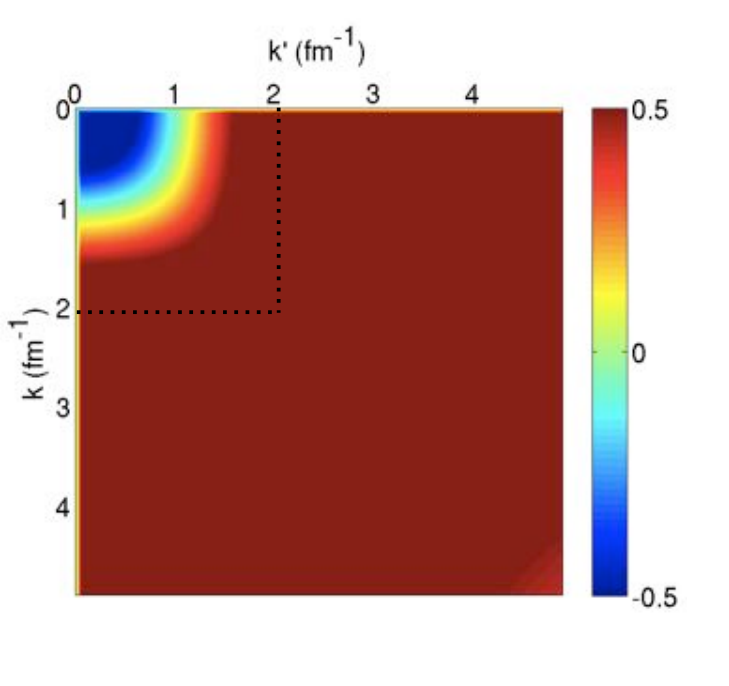
\includegraphics[width=\linewidth]{HighRes.png}
    \caption{High Resolution, before much SRG is applied}
    \label{fig:highres}
  \end{subfigure}
  \hfill
  \begin{subfigure}{0.45\textwidth}
    \centering
    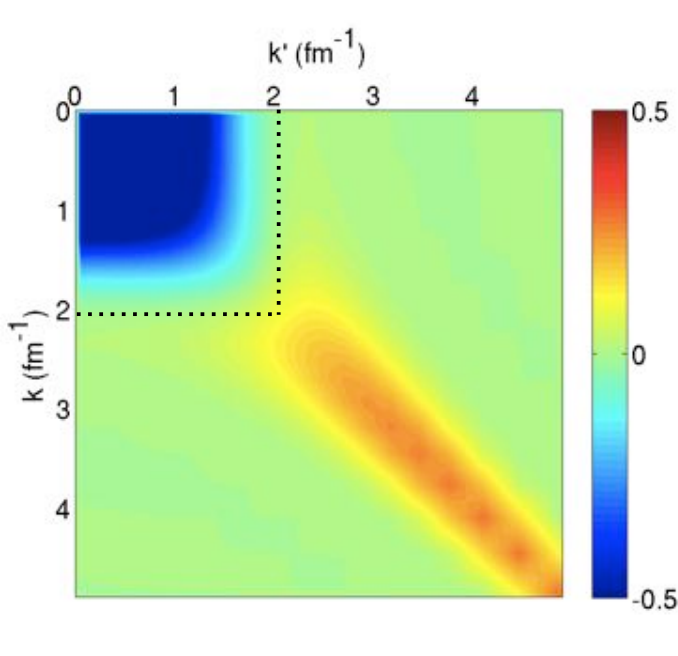
\includegraphics[width=\linewidth]{LowRes.png}
    \caption{Low Resolution after lots of SRG is applied}
    \label{fig:lowres}
  \end{subfigure}
  \caption{Nuclear potentials $V(k,k')$. Figures from Kai Hebeler:
    ``Chiral Effective Field Theory and Nuclear Forces:
    overview and applications'' presentation at TALENT school at MITP
    2022, and modified with permission from
    Furnstahl \etal \cite{Furnstahl2013}.
  }
  \label{fig:SRGtransform}
\end{figure}
In the under-evolved, high resolution figure \ref{fig:highres} the potential does 
not go to zero rapidly, whereas it does once the
transformation is applied in figure \ref{fig:lowres}. As a
result a cutoff can be made at $\LamNN=2 \mathrm{fm}^{-1}$ without
losing much accuracy whereas the under-evolved potential required at least $\LamNN=5 \mathrm{fm}^{-1}$.
The time complexity is at minimum proportional to the number of array elements
present, therefore we gain a factor of $(5/2)^2=6.25$ in efficiency;
in practice the gains are even higher.

The SRG transformation is essential, but it also creates a
change in the physical meaning of the free variables.
In fact, any unitary transformation ($U^\dag U =\mathbbm{1}$) also transforms the coordinates.
\begin{align}
  \br{p'}V\kt{p} 
  = \br{p'} U^\dag U V U^\dag U \kt{p}
  = \br{p'} U^\dag\left( U V U^\dag\right)\;U
  \kt{p}
  = \br{\widetilde{p}\,'} V_{eff}
  \kt{\widetilde{p}}=V_{eff}(\widetilde{p},\widetilde{p}\,')
\end{align}
So referring to the free variables in an SRG-transformed potential as
``momenta'' is, to some extent, incorrect.
They do not represent physical states  in the sense that they are not eigenstates to physical momenta.
The Lagrangeans that generate the Feynman diagrams in the kernel, however,
depend on physical momenta, and therefore we cannot directly use an SRG
evolved potential in the non-SRG evolved kernel.
To solve this, previous work with SRG transformations has transformed the
Lagrangeans - and therefore the kernels - into the SRG evolved space
as well\ques{get citation}.
However, in the context of the density formalism this would mean adding SRG
dependence into the kernel, thereby breaking kernel-density independence.
Additionally, the SRG transformation can take many different forms \cite{SRG, Furnstahl2013};
we wish to allow for these developments
without having to re-write the kernel code.
Therefore we have chosen to apply an inverse
transformation to the densities \cite{XiangXiang}.

The SRG evolution has parameters that must be fine-tuned, but this
allows for uncertainty estimation.
In particular, one must solve for the nucleus wavefunction; 
to this end an expansion in the harmonic oscillator basis is used.
When expanded to infinite order, this basis forms a complete set,
however, we truncate this expansion by including harmonic oscillator excitations up to $\Ntot$.
Additionally, the harmonic oscillator basis has a characteristic
width, denoted by $\omega_H$, and finally, the parameter $\LamSRG$
represents the evolution of the potential, as seen in figure
\ref{fig:SRGtransform}. $\LamSRG=\infty$ corresponds to no evolution.
All of these parameters affect the resulting cross-section.
We note that uncertainty decreases monotonically with increasing
$\Ntot$, and at $\Ntot=\infty$ the associated uncertainty goes to zero.
Applying a stronger SRG evolution (lower $\LamSRG$) to the potential results in larger
induced many-body forces; however, we show in figure \ref{fig:SRGConverge4He} the
effect of this uncertainty is small.
These induced forces exist because due to the cutoff $\LamNN$ the SRG transformation
is only approximately unitary.
Fortunately, when the TDA is calculated we also gain access to the
binding energy of the simulated system.
From this, we can estimate required values for $\omega_H$ and
$\Ntot$ by comparing the experimental binding energy to computed
binding energy.
In order to gain confidence we first applied this methodology 
to $\HeF$, where we can compare SRG and non-SRG evolved results. 
With this completed we have now moved to $\LiS$ where we only have access to 
the SRG evolved form.
\begin{figure}[H]
  \begin{center}
    \includegraphics[width=\linewidth]{
    4HeCrossSection.rel-dev-SRG-vs-nonSRG.chiralsmsN4LO+3nfN2LO-Λ550.Odelta2.pdf}
    \caption{$\HeF$\, Compton scattering SRG convergence}
    \label{fig:SRGConverge4He}
  \end{center}
\end{figure}
\begin{equation}
  \text{``Relative deviation, (Rel. deviation) of $A$ from $M$''}:=
  \frac{A}{M}-1
\end{equation}
In figure \ref{fig:SRGConverge4He}, we see the effectiveness of the
results in the $\HeF$ case.
We expect the deviation to decrease as $N$ increases, and importantly
for our analysis, this shows what value of $N$ is required.
The small error present at high $\Ntot$ is present do to the induced many body forces.\\

To estimate the uncertainty associated with the $\Ntot$ expansion, we utilize the form of 
plots as a function of $\Ntot$ and $\omega_H$.
\begin{figure}[H]
\centering
%\includegraphics[width=\linewidth]{file_path}
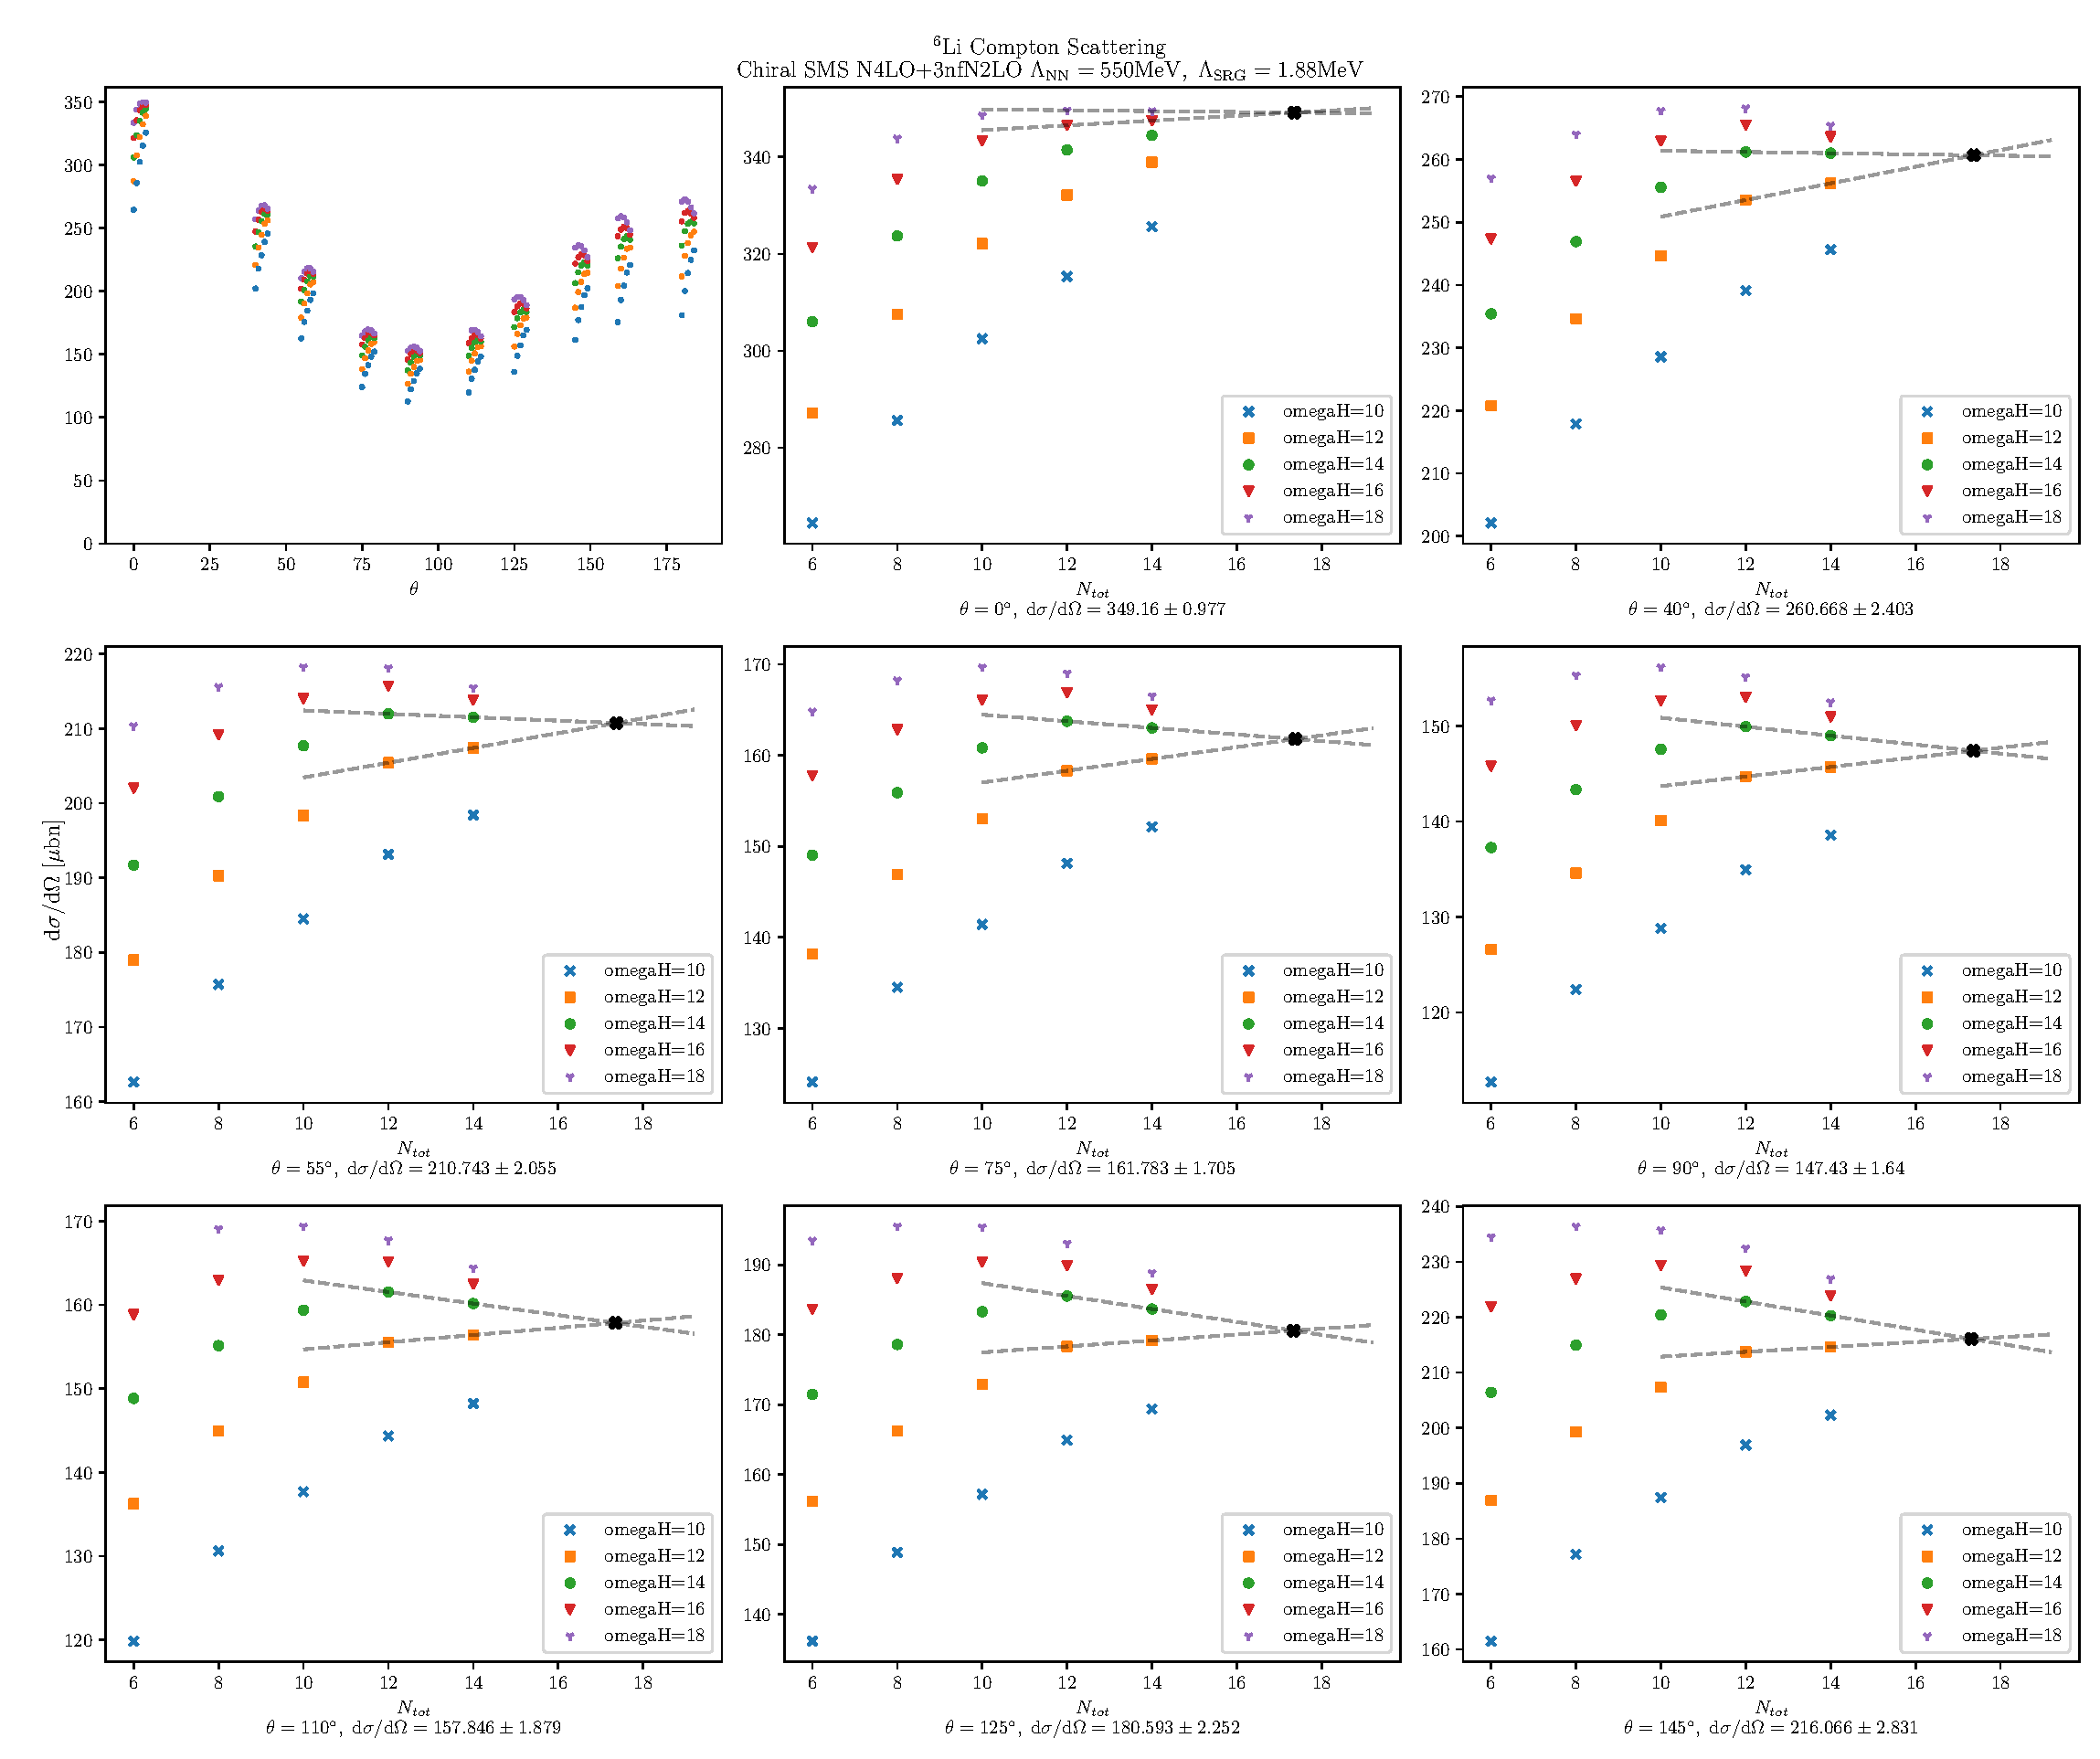
\includegraphics[width=\linewidth]{NtotmaxConverge-Lam550-SRG188.pdf}
\caption{Compton scattering on $\LiS$,}
\label{fig:Ntotuncer}
\end{figure}
First note that these values appear to be converging either from above or below depending on the value of $\omega_H$
To this end we use the squeeze theorem which grantees convergence in that range.
Considering first the values of $\omega_H$ which reproduce the binding energy most accurately ($\omega_H=14,16$), we check if we have one instance that is converging from above, and one from below.
If we do not, then we check the next available values of $\omega_H$. 
For the chosen values of $\omega_H$ let $(x, y)_{1,a},\;(x,y)_{2,a}$ be the coordinates on the points with the negative slope 
and let $(x, y)_{1,b}, (x,y)_{2,b}$ be the values of the points associated with the negative slope. Here the $x$ values are $N_{tot}$ and the $y$ values are the cross section. That is, $a$ represents one value of $\omega_H$ and $b$ another, also let $x_1<x_2$.
The reported central value comes from the intersection of the lines that interpolate the $a$ and $b$ points respectively.
The reported uncertainty is $\sigma_{N_{tot}}=|y_{2a}-y_{2b}|/2$.
Note this is only the uncertainty associated with this procedure, other forms of uncertainty contribute.

\subsection{Compton Scattering Observables in Lithium Six}
The momentum transfer $\vec{q}$ describes the transition densities,
and can be replaced by the energy of the incoming and outgoing photon
along with the scattering angle $\theta_{cm}$.
We have $\omega_{\mathrm{cm}}=|\vec{k}|=|\vec{k}'|$, and
\begin{equation}
  \cos{\theta}_{\mathrm{cm}}=1-\frac{\vec{q}^2}{2\omega_{cm}^2}
\end{equation}
The $\sixLi$ Compton cross section (with target spin $0=M=M'$) in the
lab frame is found by transferring the energies and angles from the
center of mass from using the $\sixLi$ mass of 5603.1 $\mathrm{MeV}$.
\begin{equation}
  \label{eq:crosssection}
  \frac{\dd\sigma}{\dd\Omega}=\frac{1}{6}
  \left(\frac{\omegalab^\prime}{4\pi\omegalab}\right)^2\sum\limits_{\substack{M,M'\\\lambda\,\lambda'}}
  \left|A_{M\lambda}^{M'\lambda^\prime}(\kv,\qv)\right|^2\;\;.
\end{equation}
Where the average over the spins and the polarizations give the
prefactor $\frac{1}{6} = \frac{1}{2}\cdot \frac{1}{3} $
(Why is is not $\frac{1}{2+3}$)

\color{red}
I can't find a definition of $\omegalab$ and $\omegalab^{'}$.
~\\~\\
There is one more equation about asymmetry (2.8) in the \fourHe
paper, but this sounds like it could be spin dependent, I will leave
it out for now.
\color{black}

\subsection{Compton Kernel}
\label{sec:kernels}
\color{red}
This is word for word from the \fourHe paper
\color{black}

For reviews of Compton scattering on nucleons and light nuclei in
\ChiEFT, we refer the
reader to refs.~\cite{Griesshammer:2012we, McGovern:2012ew} for
notation, relevant parts of the chiral Lagrangian, and full
references to the literature. Here, we merely summarise the power counting
and Compton kernel already employed in refs.~\cite{Hildebrandt:2005ix,
Hildebrandt:2005iw, Margaryan:2018opu} in our region of interest,
$50\;\MeV\lesssim\omega\lesssim120\;\MeV$.

When \ChiEFT with a dynamical Delta is used to compute (elastic)
Compton scattering, three low
scales compete: the pion mass $\mpi$, the Delta-nucleon mass splitting
$\DeltaM \approx 300\;\MeV$, and the photon energy $\omega$.  Each provides a
small, dimensionless expansion parameter, measured in units of the
``high'' momentum
scale $\Lambdachi$, at which the theory breaks down because new degrees of
freedom enter\footnote{This physically meaningful parameter is not to
  be confused with an unphysical ``cutoff" $\Lambda$, albeit the
symbols are similar~\cite{Furnstahl:2014xsa,Griesshammer:2021zzz}.}.
While $\frac{\mpi}{\Lambdachi}$ and
$\frac{\DeltaM}{\Lambdachi}$ have quite different chiral behaviour, we follow
Pascalutsa and Phillips~\cite{Pascalutsa:2002pi} and take a common breakdown
scale $\Lambdachi \approx 650\;\MeV$, consistent with the masses of the
$\omega$ and $\rho$ as the next-lightest exchange mesons, exploiting a
numerical coincidence at the physical pion mass to define a single
expansion parameter:
\begin{equation}
  \delta\equiv\frac{\Delta_M}{\Lambdachi}\approx \sqrt{\frac{m_\pi}{\Lambdachi}}
  \approx\sqrt{\frac{\omega}{\Lambdachi}}\approx 0.4\ll1\;\;.
\end{equation}
We also count $\MN\sim\Lambdachi$.  Since $\delta$ is not very small,
order-by-order convergence must be verified carefully, see
sect.~refsec:uncertainties.

This power counting organises contributions under the assumption
$\omega\sim\mpi$.
As extensively discussed previously~\cite{Beane:1999uq,
Beane:2004ra,Hildebrandt:2005ix, Hildebrandt:2005iw, Margaryan:2018opu} and
summarised in~\cite[sect.~5.2]{Griesshammer:2012we}, in this r\'egime
only kernels with one and
two active nucleons contribute in a \ChiEFT description of Compton
scattering up to and including
\NXLO{4} [$\calO(e^2\delta^4)$].
At lower energies $\omega \lesssim m_\pi^2/M$, this power counting
does not apply because photons with resolution $1/\omega$
larger than the size of the \fourHe nucleus scatter coherently on the whole
target.  Refs.~\cite{Hildebrandt:2005ix, Hildebrandt:2005iw,
Griesshammer:2012we} discuss in detail how the reformulated power
counting appropriate at these lower energies leads to the restoration of
the Thomson limit by inclusion of coherent propagation of the \fourHe system
in the intermediate state between absorption and emission of photons. This
rescattering effect involves the interaction of all $A$ nucleons with one
another between photon absorption and emission, and hence an $A$-body
density. However, that r\'egime is not the focus of this
presentation. Rather, we are
concerned with the non-collective contributions which dominate above about
$50\;\MeV$. That is also where data is most likely to be taken to extract
nucleon polarisabilities.

Specifically, we use the one- and two-body Compton kernels of
refs.~\cite{Bernard:1991rq,Bernard:1995dp,Beane:1999uq},
supplemented with the
$\Delta$-pole and $\pi \Delta$ loop graphs~\cite{Hildebrandt:2003fm,
Hildebrandt:2004hh, Hildebrandt:2005ix, Hildebrandt:2005iw}. They are both
conceptually and numerically identical to the ones which have been described
extensively in our Compton studies of the deuteron~\cite{Hildebrandt:2005ix,
Hildebrandt:2005iw, Griesshammer:2013vga, Myers:2014ace, Myers:2015aba}
and, most recently, \threeHe~\cite{Margaryan:2018opu,
hgrie3He}. These pieces of the photonuclear operator are
organised in a perturbative expansion which is complete up to and including
\NXLO{3} [$\calO(e^2 \delta^3)$].
No contribution enters at NLO [$\calO(e^2\delta^1)$], and only
one-body Delta contributions at \NXLO{3} [$\calO(e^2\delta^3)$]. We
only allow photon energies somewhat below
$\omega_\mathrm{thr}(\mbox{\fourHe})\approx\mpi$ in order to
avoid additional complications in the vicinity of the pion-production threshold.

The one-nucleon kernel convoluted with the one-body density as in
eq.~\eqref{eq:onebody}.

\begin{itemize}

  \item[(a)] LO [$\calO(e^2\delta^0=Q^2)$]: The single-nucleon
    (proton) Thomson term.

  \item[(b)] \NXLO{2} [$\calO(e^2\delta^2=Q^3)$] non-structure/Born terms:
    photon couplings to the nucleon charge beyond LO, to its magnetic moment, or
    to the $t$-channel exchange of a $\pi^0$ meson (irrelevant for the isoscalar
    \fourHe).

  \item[(c)] \NXLO{2} [$\calO(e^2\delta^2=Q^3)$] structure/non-Born terms:
    photon couplings to the pion cloud around the nucleon is the source of the
    LO contributions to the polarisabilities as first reported in
    refs.~\cite{Bernard:1991rq, Bernard:1995dp}.

  \item[(d/e)] \NXLO{3} [$\calO(e^2\delta^3)$] structure/non-Born terms: photon
    couplings to the pion cloud around the (non-relativistic)
    $\Delta(1232)$ (d) or
    directly exciting the Delta (e), as calculated in
    refs.~\cite{Butler:1992ci, Hemmert:1996rw, Hemmert:1997tj};
    these give NLO contributions to
    the polarisabilities. The Delta parameters are taken from
    ref.~\cite{Margaryan:2018opu}. The Delta excitation of diagram (d) shows
    considerable energy dependence even at $\omega\sim\mpi$; see the discussion
    of ``dynamical polarisabilities'' in refs.~\cite{Griesshammer:2012we,
    Griesshammer:2017txw}. This will be important in the
    interpretation of our results in sect.~ \color{red}Results\color{black}.

  \item[(f)] Short-distance/low-energy coefficients (LECs) encode those
    contributions to the nucleon polarisabilities which stem from
    physics at and above the breakdown scale $\Lambdachi$. These
    offsets to the polarisabilities are formally of higher order. We
    determine them to reproduce the isoscalar polarisabilities of
    eq.~\eqref{eq:alphabeta}. Their
    uncertainties were discussed in the Introduction  but are dwarfed
    by the other uncertainties of the results presented
    here, including those coming from the wave function dependence and higher
    order effects; see sect.~\ref{sec:uncertainties}. Neither does
    the detailed discussion of the sources and sizes
    of uncertainties of other nucleon polarisabilities in
    ref.~\cite{Griesshammer:2015ahu}
    bear on the present results. We also recall from the Introduction
    that since \fourHe is a near-perfect isoscalar and
    scalar, neither the nucleon's isovector polarisabilities nor its spin
    polarisabilities enter, except at very high orders.

\end{itemize}

%%%%%%%%%%%%%%%%%%%%%%%%%%%%%%%%%%%%%%
\begin{figure}[!t]
  \begin{center}
    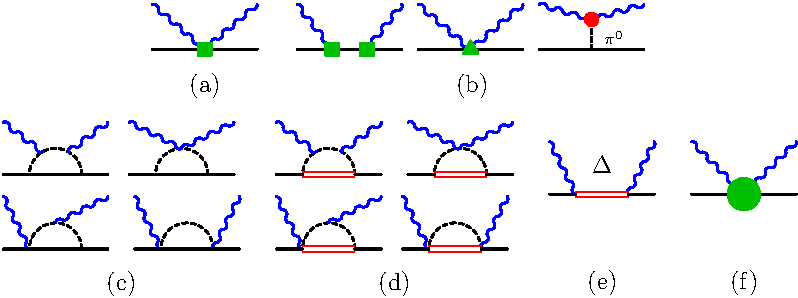
\includegraphics[width=0.8\textwidth]{figures/graphs-1B.pdf}
    \caption{(Colour on-line) The single-nucleon contributions in \ChiEFT up
      to \NXLO{3} [$\calO(e^2\delta^3)$] for
      $50\;\MeV\lesssim\omega\lesssim120\;\MeV$. The vertices are from:
      ${\cal L}_{\piN}^{(1)}$ (no symbol), ${\cal L}_{\piN}^{(2)}$ (green
      square), ${\cal L}_{\piN}^{(3)}$ (green triangle),
      ${\cal L}_{\pi\pi}^{(4)}$ (red disc)~\cite{Bernard:1995dp}; the green
      disc of graph (f) stands for variations of the polarisabilities% ,
      % cf.~eq.~\eqref{eq:fit}
      . Permuted and crossed diagrams are not
    displayed.}
    \label{fig:1Bdiagrams}
  \end{center}
\end{figure}
%%%%%%%%%%%%%%%%%%%%%%%%%%%%%%%%%%%%%%

%%%%%%%%%%%%%%%%%%%%%%%%%%%%%%%%%%%%%%
\begin{figure}[!b]
  \begin{center}
    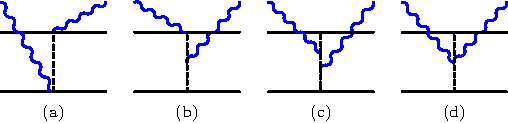
\includegraphics[width=0.5\textwidth]{figures/graphs-2B-withlabels.pdf}
    \caption{(Colour on-line) \NXLO{2} [$\calO(e^2 \delta^2)$]
      contributions to the
      (irreducible) $\gamma \N\N \rightarrow \gamma \N\N$ amplitude
      (no additional
        contributions at \NXLO{3} [$\calO(e^2 \delta^3)$].  Notation as in
      fig.~\ref{fig:1Bdiagrams}. Permuted and crossed diagrams not displayed.}
      \label{fig:2Bdiagrams}
    \end{center}
  \end{figure}
  %%%%%%%%%%%%%%%%%%%%%%%%%%%%%%%%%%%%%%

  The first nonzero two-body kernel convoluted with the two-body
  density as in eq.~\eqref{eq:twobody} enters at
  \NXLO{2} [$\calO(e^2 \delta^2)$]  and does not involve Delta
  excitations; see fig.~\ref{fig:2Bdiagrams}. It is the
  two-body analogue of the $\pi N$ loop graphs (c) in fig.~\ref{fig:1Bdiagrams},
  first computed for $t_{12}=0$ in refs.~\cite{Beane:1999uq,
  Beane:2004ra} and extended to $t_{12}=1$  in refs.~\cite{Choudhury:2007bh,
  Shukla:2008zc, ShuklaPhD} where full
  expressions can be found. These contributions are nonzero only for
  $\mathrm{np}$ pairs, that is, they all contain the same $2\N$ isospin factor.
  \begin{equation}
    \langle t_{12}m^{t\prime}_{12}|(\tau^{(1)} \cdot \tau^{(2)} -
    \tau^{(1)}_{z} \tau^{(2)}_{z})|t_{12}m^{t}_{12}\rangle=2(-1)^{t_{12}+1}\;
    \delta_{m^{t\prime}_{12}m^t_{12}}\;\delta_{m^t_{12}0}\;\;.
  \end{equation}
  Therefore, they parametrise the leading term of both photons hitting the
  charged-meson-exchange. In \fourHe, as in \threeHe, both isospin
  $t_{12}=0$ and $1$
  pairs are present. Corrections to these currents enter at one order higher,
  \NXLO{4} [$\calO(e^2\delta^4)$], than we consider here.
\subsection{Creation of Transition Probability Densities from
  Chiral Potentials}
\color{red} Again this is taken directly from the \fourHe paper \color{black}

\label{sec:potentials}

We used a class of four chiral $2$N and $3$N interactions to generate the one-
and two-body densities for \fourHe: the \ChiEFT Semi-local Momentum-Space (SMS)
$2\N$ potentials in the version ``\NXLO{4}+'' (\ie~considered to be complete at \NXLO{4} with
some \NXLO{5} interactions)~\cite{Reinert:2017usi} and the corresponding
chiral $3\N$ interaction ``\NXLO{2}'' discussed in ref.~\cite{Maris:2020qne}. We employed $2 \N$ momentum-space cutoffs $\Lambda=550\;\MeV$ (hardest),
$500\;\MeV$, $450\;\MeV$ and $400\;\MeV$ (softest) (the complete set of parameters of the 3N interactions can be found in Table~1 of Ref.~\cite{Le:2023bfj}). 
These nuclear interactions all capture the correct long-distance physics of one- and two-pion exchange and
reproduce both the $2\N$ scattering data and the experimental values of the
triton and \threeHe binding energies well. Increasing momentum cutoffs
indicate increasing ``hardness'' of the short-distance interaction. Their \fourHe binding
energies are within $+0.5\;\MeV$ ($\Lambda=550\;\MeV$) to $-0.1\;\MeV$
($\Lambda=400\;\MeV$) of the experimental value. This variation by less than $2\%$
is not a concern, since we compute for photon energies that are high enough that this slight variation in the \fourHe binding energy has no impact on the elastic Compton cross section.

These are of course but four out of a number of modern,
sophisticated potentials. Our choice is dictated by the fact that they are
semi-local (and hence of the form of AV18) and are already coded for the densities formalism. By varying the cutoff within a single family of \ChiEFT potentials, we avoid questions about how the cutoffs of different realisations of the \ChiEFT regulator functions are related. The range of cutoffs chosen, while not large enough to establish renormalisability of the theory, is large enough to indicate a lower bound of the sensitivity of cross sections to the short-distance physics of this process. 

These \ChiEFT wave functions use Weinberg's ``hybrid
approach''~\cite{Weinberg:1990rz}, in which potentials are derived to an assumed
accuracy and then iterated to produce amplitudes or, in our case, one- and
two-body densities. All claim a higher accuracy than that of our Compton
kernels. We refrain here from entering the ongoing debate about correct implementations
of the chiral power counting or the range of cutoff variations, etc.; see
refs.~\cite{Phillips:2013fia, vanKolck:2020llt} for concise summaries, ref.~\cite{Griesshammer:2021zzz} for a polemic, and ref.~\cite{Tews:2022yfb} for a variety of community voices.

Similarly, even though the Compton Ward identities are violated because the
one-pion-exchange $2\N$ potentials are regulated, any inconsistencies between
currents and nuclear densities is compensated by operators which enter at
higher orders in \ChiEFT than the last order we fully retain [\NXLO{3},
$\calO(e^2\delta^3)$]. In addition, the potentials do not include explicit
Delta contributions while the kernel does.  However, it is easy to see that,
for real Compton scattering around $120\;\MeV$, a Delta excited directly by
the incoming photon is more important than one that occurs virtually between
exchanges of virtual pions, especially for an isoscalar target like
\fourHe. For our purposes, such Delta excitations in the $2\N$ potential are
already suppressed by several orders in the chiral counting and well
approximated by the $\pi N$ seagull Low Energy Coefficients that enter the \NXLO{3} interaction.

 sect.~\ref{sec:dependence-pots}, we therefore take the differences between results with the $4$ 
fferent sets of densities as providing a lower bound indicative of the
esent residual theoretical uncertainties. These do not affect the
nclusions of our sensitivity studies, but better extractions of
larisabilities from \fourHe data will undoubtedly need a reduced potential
spread. 
The results generated with the potential \chiSMSfourfive turn out to be approximately the mean of those generated from the different potentials considered, so we use that for central values, and assess variations with respect to it. 

The \fourHe one- and two-body densities, together with the \threeHe
densities, are publicly available
using the python package provided at~\url{ https://pypi.org/project/nucdens/}. They are defined in momentum space, for centre-of-mass energies and
momentum transfers corresponding to Compton scattering photon energies between
$\omegacm=50$ and $120\;\MeV$ in steps of $10\;\MeV$ and scattering angles
$\thetacm\in[0;180^\circ]$ in steps of $15^\circ$ (momentum-transfers
$\sqrt{\qv^2}\in[0;240]\;\MeV$), plus at selected higher and lower energies
for control. Also available are densities using the harder AV18 $2\N$ model
interaction~\cite{Wiringa:1994wb}, supplemented by the Urbana-IX $3\N$
interaction (3NI)~\cite{Pudliner:1995wk, Pudliner:1997ck}, and densities using the chiral Idaho interaction for
the $2\N$ system in the version ``\NXLO{3}'' at cutoff
$500\;\MeV$~\cite{Entem:2003ft} with the \ChiEFT $3\N$ interaction in the
version ``$\calO(Q^3)$'' using variant ``b'' of
ref.~\cite{Nogga:2005hp} as the ``softest'' choice. 

  \section{Results}
  \subsection{Differential Cross Section}
  Differential cross section plot here
  \subsection{Comparison to Experimental Data}
  Gerry's data goes here
  \subsection{Uncertainty Analysis}
  \label{sec:uncertainties}
  Bayesian approach blah blah blah
  \subsubsection{A-Priori estimate}
  \ques{What is this?}

  \subsubsection{Convergence of the Chiral EFT Expansion}
  Show convergence order by order
  \subsubsection{SRG Induced Many-Body Forces}
  Compare to \fourHe maybe?
  \subsubsection{Residual Dependence on the 2N and 3N Interactions}
  \subsubsection{Numerical Uncertainty}
  \subsubsection{Total Uncertainty}
  Plot about dependence on $\al,\be$
  \subsection{Sensitivity to the Scalar-Isoscalar Polarisabilities}
  \subsection{Beam Asymmetry}
  Plots here
  \subsection{Comparison with Other Few Nucleon Targets}
  Plot of ratios here
  \section{Summary and Conclusions}
\begin{thebibliography}{44}

\bibitem{Nogga:2005hp} 
A.~Nogga, P.~Navrátil, B.~R. Barrett, and J.~P. Vary, 
``Spectra and binding energy predictions of chiral interactions for ${}^7\mathrm{Li}$,''\\ 
\textit{Physical Review C} \textbf{73} (2006) 064002.\\ 
DOI: \href{http://dx.doi.org/10.1103/PhysRevC.73.064002}{10.1103/PhysRevC.73.064002}.

\bibitem{Entem:2003ft} 
D.~R. Entem and R. Machleidt, 
``Accurate charge-dependent nucleon-nucleon potential at fourth order of chiral perturbation theory,''\\ 
\textit{Physical Review C} \textbf{68} (2003) 041001.\\ 
DOI: \href{http://dx.doi.org/10.1103/PhysRevC.68.041001}{10.1103/PhysRevC.68.041001}.

\bibitem{Pudliner:1997ck} 
B.~S. Pudliner, V.~R. Pandharipande, J. Carlson, S.~C. Pieper, and R.~B. Wiringa, 
``Quantum Monte Carlo calculations of nuclei with $A\leq7$,''\\ 
\textit{Physical Review C} \textbf{56} (1997) 1720–1750.\\ 
DOI: \href{http://dx.doi.org/10.1103/PhysRevC.56.1720}{10.1103/PhysRevC.56.1720}.

\bibitem{Pudliner:1995wk} 
B.~S. Pudliner, V.~R. Pandharipande, J. Carlson, and R.~B. Wiringa, 
``Quantum Monte Carlo Calculations of $A\leq6$ Nuclei,''\\ 
\textit{Physical Review Letters} \textbf{74} (1995) 4396–4399.\\ 
DOI: \href{http://dx.doi.org/10.1103/physrevlett.74.4396}{10.1103/physrevlett.74.4396}.

\bibitem{Wiringa:1994wb} 
R.~B. Wiringa, V.~G.~J. Stoks, and R. Schiavilla, 
``Accurate nucleon-nucleon potential with charge-independence breaking,''\\ 
\textit{Physical Review C} \textbf{51} (1995) 38–51.\\ 
DOI: \href{http://dx.doi.org/10.1103/physrevc.51.38}{10.1103/physrevc.51.38}.

\bibitem{Tews:2022yfb} 
Ingo Tews \textit{et al.}, 
``Nuclear Forces for Precision Nuclear Physics: A Collection of Perspectives,''\\ 
\textit{Few-Body Systems} \textbf{63} (2022).\\ 
DOI: \href{http://dx.doi.org/10.1007/s00601-022-01749-x}{10.1007/s00601-022-01749-x}.

\bibitem{vanKolck:2020llt} 
U.~van Kolck, 
``The Problem of Renormalization of Chiral Nuclear Forces,''\\ 
arXiv:2003.06721 (2020). Available at: \url{https://arxiv.org/abs/2003.06721}.

\bibitem{Reinert:2017usi} 
P.~Reinert, H.~Krebs, and E.~Epelbaum, 
``Semilocal momentum-space regularized chiral two-nucleon potentials up to fifth order,''\\ 
\textit{The European Physical Journal A} \textbf{54} (2018) Article 12516.\\ 
DOI: \href{http://dx.doi.org/10.1140/epja/i2018-12516-4}{10.1140/epja/i2018-12516-4}.

\bibitem{Phillips:2013fia} 
D.~R. Phillips, 
``Recent results in chiral effective field theory for the NN system,''\\ 
arXiv:1302.5959 (2013). Available at: \url{https://arxiv.org/abs/1302.5959}.

\bibitem{Weinberg:1990rz} 
S.~Weinberg, 
``Nuclear forces from chiral lagrangians,''\\ 
\textit{Physics Letters B} \textbf{251} (1990) 288–292.\\ 
DOI: \href{https://doi.org/10.1016/0370-2693(90)90938-3}{10.1016/0370-2693(90)90938-3}.

\bibitem{Le:2023bfj} 
H.~Le, J.~Haidenbauer, U.~G. Mei\ss{}ner, and A.~Nogga, 
``Separation energies of light $\Lambda$ hypernuclei and their theoretical uncertainties,''\\ 
arXiv:2308.01756, DOI: \href{https://doi.org/10.1140/epja/s10050-023-01219-w}{10.1140/epja/s10050-023-01219-w}.

\bibitem{Maris:2020qne} 
P.~Maris \textit{et al.} (Lenpic Collaboration), 
``Light nuclei with semilocal momentum-space regularized chiral interactions up to third order,''\\ 
\textit{Physical Review C} \textbf{103} (2021) 054001.\\ 
DOI: \href{http://dx.doi.org/10.1103/PhysRevC.103.054001}{10.1103/PhysRevC.103.054001}.

\bibitem{ShuklaPhD} 
D.~Shukla, 
``Investigating Neutron Polarizabilities and NN Scattering in Heavy-Baryon Chiral Perturbation Theory,''\\ 
Ph.D. thesis. Available at: \url{http://rave.ohiolink.edu/etdc/view?acc_num=ohiou1163711618}.

\bibitem{Shukla:2008zc} 
D.~Shukla, A.~Nogga, and D.~R. Phillips, 
``Analyzing the effects of neutron polarizabilities in elastic Compton scattering off $^3$He,''\\ 
\textit{Nuclear Physics A} \textbf{819} (2009) 98–134.\\ 
DOI: \href{http://dx.doi.org/10.1016/j.nuclphysa.2009.01.003}{10.1016/j.nuclphysa.2009.01.003}.

\bibitem{Hemmert:1997tj} 
T.~R. Hemmert, B.~R. Holstein, J.~Kambor, and G.~Knöchlein, 
``Compton scattering and the spin structure of the nucleon at low energies,''\\ 
\textit{Physical Review D} \textbf{57} (1998) 5746–5754.\\ 
DOI: \href{http://dx.doi.org/10.1103/physrevd.57.5746}{10.1103/physrevd.57.5746}.

\bibitem{Griesshammer:2017txw} 
H.~W. Grießhammer, J.~A. McGovern, and D.~R. Phillips, 
``Comprehensive study of observables in Compton scattering on the nucleon,''\\ 
\textit{The European Physical Journal A} \textbf{54} (2018) Article 12467.\\ 
DOI: \href{http://dx.doi.org/10.1140/epja/i2018-12467-8}{10.1140/epja/i2018-12467-8}.

\bibitem{Choudhury:2007bh} 
D.~Choudhury, A.~Nogga, and D.~R. Phillips, 
``Investigating Neutron Polarizabilities through Compton Scattering on $^3$He,''\\ 
\textit{Physical Review Letters} \textbf{98} (2007) 232303.\\ 
DOI: \href{http://dx.doi.org/10.1103/physrevlett.98.232303}{10.1103/physrevlett.98.232303}.

\bibitem{Butler:1992ci} 
M.~N. Butler and M.~J. Savage, 
``Electromagnetic polarisability of the nucleon in chiral perturbation theory,''\\ 
\textit{Physics Letters B} \textbf{294} (1992) 369–374.\\ 
DOI: \href{http://dx.doi.org/10.1016/0370-2693(92)91535-h}{10.1016/0370-2693(92)91535-h}.

\bibitem{Hemmert:1996rw} 
T.~R. Hemmert, B.~R. Holstein, and J.~Kambor, 
``Delta(1232) and the Polarizabilities of the Nucleon,''\\ 
\textit{Physical Review D} \textbf{55} (1997) 5598–5612.\\ 
DOI: \href{http://dx.doi.org/10.1103/physrevd.55.5598}{10.1103/physrevd.55.5598}.

\bibitem{Myers:2015aba} 
L.~S. Myers \textit{et al.}, 
``Compton scattering from the deuteron below pion-production threshold,''\\ 
\textit{Physical Review C} \textbf{92} (2015) 025203.\\ 
DOI: \href{http://dx.doi.org/10.1103/physrevc.92.025203}{10.1103/physrevc.92.025203}.

\bibitem{Myers:2014ace} 
L.~S. Myers \textit{et al.}, 
``Measurement of Compton Scattering from the Deuteron and an Improved Extraction of the Neutron Electromagnetic Polarizabilities,''\\ 
\textit{Physical Review Letters} \textbf{113} (2014) 262506.\\ 
DOI: \href{http://dx.doi.org/10.1103/physrevlett.113.262506}{10.1103/physrevlett.113.262506}.

\bibitem{Griesshammer:2013vga} 
H.~W. Grießhammer, 
``Dissecting deuteron Compton scattering I: The observables with polarised initial states,''\\ 
\textit{European Physical Journal A}.\\ 
DOI: \href{https://doi.org/10.1140/epja/i2013-13100-2}{10.1140/epja/i2013-13100-2}. 
(Note: Detailed volume and year information was not provided in the original entry.)

\bibitem{Hildebrandt:2003fm} 
R.~P. Hildebrandt, H.~W. Grießhammer, T.~R. Hemmert, and B.~Pasquini, 
``Signatures of chiral dynamics in low-energy Compton scattering off the nucleon,''\\ 
\textit{The European Physical Journal A} \textbf{20} (2004) 293–315.\\ 
DOI: \href{http://dx.doi.org/10.1140/epja/i2003-10144-9}{10.1140/epja/i2003-10144-9}.

\bibitem{Hildebrandt:2004hh} 
R.~P. Hildebrandt, H.~W. Grießhammer, T.~R. Hemmert, and D.~R. Phillips, 
``Explicit $\Delta(1232)$ degrees of freedom in Compton scattering off the deuteron,''\\ 
\textit{Nuclear Physics A} \textbf{748} (2005) 573–595.\\ 
DOI: \href{https://doi.org/10.1016/j.nuclphysa.2004.11.017}{10.1016/j.nuclphysa.2004.11.017}.

\bibitem{Bernard:1995dp} 
V.~Bernard, N.~Kaiser, and Ulf-G. Meißner, 
``Chiral dynamics in nucleons and nuclei,''\\ 
\textit{International Journal of Modern Physics E} \textbf{4}, no. 2 (1995) 193–344.\\ 
DOI: \href{http://dx.doi.org/10.1142/s0218301395000092}{10.1142/s0218301395000092}.

\bibitem{Bernard:1991rq} 
V.~Bernard, N.~Kaiser, and Ulf-G. Meißner, 
``Chiral expansion of the nucleon's electromagnetic polarizabilities,''\\ 
\textit{Physical Review Letters} \textbf{67} (1991) 1515–1518.\\ 
DOI: \href{http://dx.doi.org/10.1103/PhysRevLett.67.1515}{10.1103/PhysRevLett.67.1515}.

\bibitem{Griesshammer:2021zzz} 
H.~W. Grießhammer, 
``What Can Possibly Go Wrong?,''\\ 
\textit{Few-Body Systems} \textbf{63} (2022) Article 01739-z.\\ 
DOI: \href{http://dx.doi.org/10.1007/s00601-022-01739-z}{10.1007/s00601-022-01739-z}.

\bibitem{Furnstahl:2014xsa} 
R.~J. Furnstahl, D.~R. Phillips, and S. Wesolowski, 
``A recipe for EFT uncertainty quantification in nuclear physics,''\\ 
\textit{Journal of Physics G: Nuclear and Particle Physics} \textbf{42} (2015) 034028.\\ 
DOI: \href{http://dx.doi.org/10.1088/0954-3899/42/3/034028}{10.1088/0954-3899/42/3/034028}.

\bibitem{Pascalutsa:2002pi} 
V.~Pascalutsa and D.~R. Phillips, 
``Effective theory of the Delta(1232) resonance in Compton scattering off the nucleon,''\\ 
\textit{Physical Review C} \textbf{67} (2003) 055202.\\ 
DOI: \href{http://dx.doi.org/10.1103/physrevc.67.055202}{10.1103/physrevc.67.055202}.

\bibitem{Beane:2004ra} 
S.~R. Beane, M.~Malheiro, J.~A. McGovern, D.~R. Phillips, and U.~van Kolck, 
``Compton scattering on the proton, neutron, and deuteron in chiral perturbation theory,''\\ 
\textit{Nuclear Physics A} \textbf{747} (2005) 311–361.\\ 
DOI: \href{http://dx.doi.org/10.1016/j.nuclphysa.2004.09.068}{10.1016/j.nuclphysa.2004.09.068}.

\bibitem{Beane:1999uq} 
S.~R. Beane, M.~Malheiro, D.~R. Phillips, and U.~van Kolck, 
``Compton scattering on the deuteron in baryon chiral perturbation theory,''\\ 
\textit{Nuclear Physics A} \textbf{656} (1999) 367–399.\\ 
DOI: \href{http://dx.doi.org/10.1016/s0375-9474(99)00312-7}{10.1016/s0375-9474(99)00312-7}.

\bibitem{Hildebrandt:2005iw} 
R.~P. Hildebrandt, H.~W. Grießhammer, and T.~R. Hemmert, 
``Nucleon polarizabilities from deuteron Compton scattering within a Green’s function hybrid approach,''\\ 
\textit{The European Physical Journal A} \textbf{46} (2010) 111–137.\\ 
DOI: \href{http://dx.doi.org/10.1140/epja/i2010-11024-y}{10.1140/epja/i2010-11024-y}.

\bibitem{Hildebrandt:2005ix} 
R.~P. Hildebrandt, 
``Elastic Compton Scattering from the Nucleon and Deuteron,''\\ 
arXiv:nucl-th/0512064 (2005). Available at: \url{https://arxiv.org/abs/nucl-th/0512064}.

\bibitem{Margaryan:2018opu} 
A.~Margaryan, B.~Strandberg, H.~W. Grießhammer, J.~A. McGovern, D.~R. Phillips, and D.~Shukla, 
``Elastic Compton scattering from $^3$He and the role of the Delta,''\\ 
\textit{The European Physical Journal A} \textbf{54} (2018) Article 12554.\\ 
DOI: \href{http://dx.doi.org/10.1140/epja/i2018-12554-x}{10.1140/epja/i2018-12554-x}.

\bibitem{McGovern:2012ew} 
J.~A. McGovern, D.~R. Phillips, and H.~W. Grießhammer, 
``Compton scattering from the proton in an effective field theory with explicit Delta degrees of freedom,''\\ 
\textit{The European Physical Journal A} \textbf{49} (2013) 13012–1.\\ 
DOI: \href{http://dx.doi.org/10.1140/epja/i2013-13012-1}{10.1140/epja/i2013-13012-1}.

\bibitem{Griesshammer:2012we} 
H.~W. Grießhammer, J.~A. McGovern, D.~R. Phillips, and G.~Feldman, 
``Using Effective Field Theory to analyse low-energy Compton scattering data from protons and light nuclei,''\\ 
\textit{Progress in Particle and Nuclear Physics} \textbf{67} (2012) 841–897.\\ 
DOI: \href{http://dx.doi.org/10.1016/j.ppnp.2012.04.003}{10.1016/j.ppnp.2012.04.003}.

\bibitem{dm_density} 
J.~de Vries, C.~Köber, A.~Nogga, and S.~Shain, 
``Dark matter scattering off ${}^4$He in chiral effective field theory,''\\ 
arXiv:2310.11343 (2023). Available at: \url{https://arxiv.org/abs/2310.11343}.

\bibitem{Griesshammer:2015ahu} 
H.~W. Grießhammer, J.~A. McGovern, and D.~R. Phillips, 
``Nucleon polarisabilities at and beyond physical pion masses,''\\ 
\textit{The European Physical Journal A} \textbf{52} (2016) Article 16139–5.\\ 
DOI: \href{http://dx.doi.org/10.1140/epja/i2016-16139-5}{10.1140/epja/i2016-16139-5}.

\bibitem{Myers_2015} 
L.~S. Myers \textit{et al.}, 
``Compton scattering from the deuteron below pion-production threshold,''\\ 
\textit{Physical Review C} \textbf{92} (2015) 025203.\\ 
DOI: \href{http://dx.doi.org/10.1103/physrevc.92.025203}{10.1103/physrevc.92.025203}.

\bibitem{Myers_2014} 
L.~S. Myers \textit{et al.}, 
``Measurement of Compton Scattering from the Deuteron and an Improved Extraction of the Neutron Electromagnetic Polarizabilities,''\\ 
\textit{Physical Review Letters} \textbf{113} (2014) 262506.\\ 
DOI: \href{http://dx.doi.org/10.1103/physrevlett.113.262506}{10.1103/physrevlett.113.262506}.

\bibitem{hgrie4He} 
H.~W. Grießhammer, J.~Liao, J.~A. McGovern, A.~Nogga, and D.~R. Phillips, 
``Compton Scattering on $^4$He with Nuclear One- and Two-Body Densities,''\\ 
arXiv:2401.16995 (2024). Available at: \url{https://arxiv.org/abs/2401.16995}.

\bibitem{60MeV} 
L.~S. Myers, M.~W. Ahmed, G.~Feldman, S.~S. Henshaw, M.~A. Kovash, J.~M. Mueller, and H.~R. Weller, 
``Compton scattering from Li-6 at 60 MeV,''\\ 
\textit{Physical Review C} \textbf{86} (2012) 044614.\\ 
DOI: \href{https://doi.org/10.1103/PhysRevC.86.044614}{10.1103/PhysRevC.86.044614}.

\bibitem{86MeV} 
L.~S. Myers, M.~W. Ahmed, G.~Feldman, A.~Kafkarkou, D.~P. Kendellen, I.~Mazumdar, J.~M. Mueller, M.~H. Sikora, H.~R. Weller, and W.~R. Zimmerman, 
``Compton Scattering from $^6$Li at 86 MeV,''\\ 
\textit{Physical Review C} \textbf{90} (2014) 027603.\\ 
DOI: \href{https://doi.org/10.1103/PhysRevC.90.027603}{10.1103/PhysRevC.90.027603}.

\bibitem{hgrie3He} 
H.~W. Grießhammer, J.~A. McGovern, A.~Nogga, and D.~R. Phillips, 
``Scattering Observables from One- and Two-body Densities: Formalism and Application to $^3$He Scattering,''\\ 
\textit{Few-Body Systems} \textbf{61} (2020) Article 01578–w.\\ 
DOI: \href{http://dx.doi.org/10.1007/s00601-020-01578-w}{10.1007/s00601-020-01578-w}.

\bibitem{SRG}
S. Szpigel and R. J. Perry, ``The Similarity Renormalization Group,'', Quantum Field Theory: A Twentieth Century Profile,

\bibitem{Furnstahl2013}
R. J. Furnstahl and K. Hebeler, ``New applications of
renormalization group methods in nuclear physics,'' \textit{Reports
on Progress in Physics}, vol. 76, no. 12, p. 126301, Nov. 2013.
DOI:
\href{http://dx.doi.org/10.1088/0034-4885/76/12/126301}{10.1088/0034-4885/76/12/126301}.
\bibitem{XiangXiang}
X.-X. Sun, H. Le, A. Nogga, and U.-G. Meißner, in preparation (2025).

\bibitem{Reinert2018}
P. Reinert, H. Krebs, and E. Epelbaum, ``Semilocal momentum-space
regularized chiral two-nucleon potentials up to fifth order,''
\textit{The European Physical Journal A}, vol. 54, no. 5, May 2018.
DOI:
\href{http://dx.doi.org/10.1140/epja/i2018-12516-4}{10.1140/epja/i2018-12516-4}.
\end{thebibliography}
\end{document}
